\documentclass[12pt,a4paper]{report}
\usepackage{graphicx,iman,extra,ttbox,pdfsetup}

\title{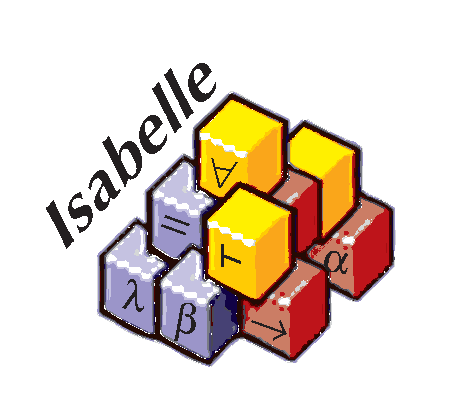
\includegraphics[scale=0.5]{isabelle} \\[4ex] Old Isabelle Reference Manual}

\author{{\em Lawrence C. Paulson}\\
        Computer Laboratory \\ University of Cambridge \\
        \texttt{lcp@cl.cam.ac.uk}\\[3ex] 
        With Contributions by Tobias Nipkow and Markus Wenzel}  

\setcounter{secnumdepth}{2} \setcounter{tocdepth}{2}

\pagestyle{headings}
\sloppy
\binperiod     %%%treat . like a binary operator

\begin{document}
\underscoreoff

\index{definitions|see{rewriting, meta-level}}
\index{rewriting!object-level|see{simplification}}
\index{meta-rules|see{meta-rules}}

\maketitle 
\emph{Note}: this document is part of the earlier Isabelle
documentation and is mostly outdated.  Fully obsolete parts of the
original text have already been removed.  The remaining material
covers some aspects that did not make it into the newer manuals yet
\cite{isabelle-isar-ref,isabelle-implementation}.

\subsubsection*{Acknowledgements} 
Tobias Nipkow, of T. U. Munich, wrote most of
  Chapters~\protect\ref{Defining-Logics} and~\protect\ref{chap:simplification}.
  Markus Wenzel contributed to Chapter~\protect\ref{chap:syntax}.
  Jeremy Dawson, Sara Kalvala, Martin
  Simons  and others suggested changes
  and corrections.  The research has been funded by the EPSRC (grants
  GR/G53279, GR/H40570, GR/K57381, GR/K77051, GR/M75440) and by ESPRIT
  (projects 3245: Logical Frameworks, and 6453: Types), and by the DFG
  Schwerpunktprogramm \emph{Deduktion}.

\pagenumbering{roman} \tableofcontents \clearfirst

%% $Id$
\chapter{Theorems and Forward Proof}
\index{theorems|(}

Theorems, which represent the axioms, theorems and rules of object-logics,
have type \mltydx{thm}.  This chapter begins by describing operations that
print theorems and that join them in forward proof.  Most theorem
operations are intended for advanced applications, such as programming new
proof procedures.  Many of these operations refer to signatures, certified
terms and certified types, which have the \ML{} types {\tt Sign.sg}, {\tt
  Sign.cterm} and {\tt Sign.ctyp} and are discussed in
Chapter~\ref{theories}.  Beginning users should ignore such complexities
--- and skip all but the first section of this chapter.

The theorem operations do not print error messages.  Instead, they raise
exception~\xdx{THM}\@.  Use \ttindex{print_exn} to display
exceptions nicely:
\begin{ttbox} 
allI RS mp  handle e => print_exn e;
{\out Exception THM raised:}
{\out RSN: no unifiers -- premise 1}
{\out (!!x. ?P(x)) ==> ALL x. ?P(x)}
{\out [| ?P --> ?Q; ?P |] ==> ?Q}
{\out}
{\out uncaught exception THM}
\end{ttbox}


\section{Basic operations on theorems}
\subsection{Pretty-printing a theorem}
\index{theorems!printing of}
\begin{ttbox} 
prth          : thm -> thm
prths         : thm list -> thm list
prthq         : thm Sequence.seq -> thm Sequence.seq
print_thm     : thm -> unit
print_goals   : int -> thm -> unit
string_of_thm : thm -> string
\end{ttbox}
The first three commands are for interactive use.  They are identity
functions that display, then return, their argument.  The \ML{} identifier
{\tt it} will refer to the value just displayed.

The others are for use in programs.  Functions with result type {\tt unit}
are convenient for imperative programming.

\begin{ttdescription}
\item[\ttindexbold{prth} {\it thm}]  
prints {\it thm\/} at the terminal.

\item[\ttindexbold{prths} {\it thms}]  
prints {\it thms}, a list of theorems.

\item[\ttindexbold{prthq} {\it thmq}]  
prints {\it thmq}, a sequence of theorems.  It is useful for inspecting
the output of a tactic.

\item[\ttindexbold{print_thm} {\it thm}]  
prints {\it thm\/} at the terminal.

\item[\ttindexbold{print_goals} {\it limit\/} {\it thm}]  
prints {\it thm\/} in goal style, with the premises as subgoals.  It prints
at most {\it limit\/} subgoals.  The subgoal module calls {\tt print_goals}
to display proof states.

\item[\ttindexbold{string_of_thm} {\it thm}]  
converts {\it thm\/} to a string.
\end{ttdescription}


\subsection{Forward proof: joining rules by resolution}
\index{theorems!joining by resolution}
\index{resolution}\index{forward proof}
\begin{ttbox} 
RSN : thm * (int * thm) -> thm                 \hfill{\bf infix}
RS  : thm * thm -> thm                         \hfill{\bf infix}
MRS : thm list * thm -> thm                    \hfill{\bf infix}
RLN : thm list * (int * thm list) -> thm list  \hfill{\bf infix}
RL  : thm list * thm list -> thm list          \hfill{\bf infix}
MRL : thm list list * thm list -> thm list     \hfill{\bf infix}
\end{ttbox}
Joining rules together is a simple way of deriving new rules.  These
functions are especially useful with destruction rules.  To store
the result in the theorem database, use \ttindex{bind_thm}
(\S\ref{ExtractingAndStoringTheProvedTheorem}). 
\begin{ttdescription}
\item[\tt$thm@1$ RSN $(i,thm@2)$] \indexbold{*RSN} 
  resolves the conclusion of $thm@1$ with the $i$th premise of~$thm@2$.
  Unless there is precisely one resolvent it raises exception
  \xdx{THM}; in that case, use {\tt RLN}.

\item[\tt$thm@1$ RS $thm@2$] \indexbold{*RS} 
abbreviates \hbox{\tt$thm@1$ RSN $(1,thm@2)$}.  Thus, it resolves the
conclusion of $thm@1$ with the first premise of~$thm@2$.

\item[\tt {$[thm@1,\ldots,thm@n]$} MRS $thm$] \indexbold{*MRS} 
  uses {\tt RSN} to resolve $thm@i$ against premise~$i$ of $thm$, for
  $i=n$, \ldots,~1.  This applies $thm@n$, \ldots, $thm@1$ to the first $n$
  premises of $thm$.  Because the theorems are used from right to left, it
  does not matter if the $thm@i$ create new premises.  {\tt MRS} is useful
  for expressing proof trees.

\item[\tt$thms@1$ RLN $(i,thms@2)$] \indexbold{*RLN} 
  joins lists of theorems.  For every $thm@1$ in $thms@1$ and $thm@2$ in
  $thms@2$, it resolves the conclusion of $thm@1$ with the $i$th premise
  of~$thm@2$, accumulating the results. 

\item[\tt$thms@1$ RL $thms@2$] \indexbold{*RL} 
abbreviates \hbox{\tt$thms@1$ RLN $(1,thms@2)$}. 

\item[\tt {$[thms@1,\ldots,thms@n]$} MRL $thms$] \indexbold{*MRL} 
is analogous to {\tt MRS}, but combines theorem lists rather than theorems.
It too is useful for expressing proof trees.
\end{ttdescription}


\subsection{Expanding definitions in theorems}
\index{meta-rewriting!in theorems}
\begin{ttbox} 
rewrite_rule       : thm list -> thm -> thm
rewrite_goals_rule : thm list -> thm -> thm
\end{ttbox}
\begin{ttdescription}
\item[\ttindexbold{rewrite_rule} {\it defs} {\it thm}]  
unfolds the {\it defs} throughout the theorem~{\it thm}.

\item[\ttindexbold{rewrite_goals_rule} {\it defs} {\it thm}]  
unfolds the {\it defs} in the premises of~{\it thm}, but leaves the
conclusion unchanged.  This rule underlies \ttindex{rewrite_goals_tac}, but 
serves little purpose in forward proof.
\end{ttdescription}


\subsection{Instantiating a theorem}
\index{instantiation}
\begin{ttbox}
read_instantiate    :            (string*string)list -> thm -> thm
read_instantiate_sg : Sign.sg -> (string*string)list -> thm -> thm
cterm_instantiate   :    (Sign.cterm*Sign.cterm)list -> thm -> thm
\end{ttbox}
These meta-rules instantiate type and term unknowns in a theorem.  They are
occasionally useful.  They can prevent difficulties with higher-order
unification, and define specialized versions of rules.
\begin{ttdescription}
\item[\ttindexbold{read_instantiate} {\it insts} {\it thm}] 
processes the instantiations {\it insts} and instantiates the rule~{\it
thm}.  The processing of instantiations is described
in \S\ref{res_inst_tac}, under {\tt res_inst_tac}.  

Use {\tt res_inst_tac}, not {\tt read_instantiate}, to instantiate a rule
and refine a particular subgoal.  The tactic allows instantiation by the
subgoal's parameters, and reads the instantiations using the signature
associated with the proof state.

Use {\tt read_instantiate_sg} below if {\it insts\/} appears to be treated
incorrectly.

\item[\ttindexbold{read_instantiate_sg} {\it sg} {\it insts} {\it thm}]
  resembles \hbox{\tt read_instantiate {\it insts} {\it thm}}, but reads
  the instantiations under signature~{\it sg}.  This is necessary to
  instantiate a rule from a general theory, such as first-order logic,
  using the notation of some specialized theory.  Use the function {\tt
    sign_of} to get a theory's signature.

\item[\ttindexbold{cterm_instantiate} {\it ctpairs} {\it thm}] 
is similar to {\tt read_instantiate}, but the instantiations are provided
as pairs of certified terms, not as strings to be read.
\end{ttdescription}


\subsection{Miscellaneous forward rules}\label{MiscellaneousForwardRules}
\index{theorems!standardizing}
\begin{ttbox} 
standard         :           thm -> thm
zero_var_indexes :           thm -> thm
make_elim        :           thm -> thm
rule_by_tactic   : tactic -> thm -> thm
\end{ttbox}
\begin{ttdescription}
\item[\ttindexbold{standard} $thm$]  
puts $thm$ into the standard form of object-rules.  It discharges all
meta-assumptions, replaces free variables by schematic variables, and
renames schematic variables to have subscript zero.

\item[\ttindexbold{zero_var_indexes} $thm$] 
makes all schematic variables have subscript zero, renaming them to avoid
clashes. 

\item[\ttindexbold{make_elim} $thm$] 
\index{rules!converting destruction to elimination}
converts $thm$, a destruction rule of the form $\List{P@1;\ldots;P@m}\Imp
Q$, to the elimination rule $\List{P@1; \ldots; P@m; Q\Imp R}\Imp R$.  This
is the basis for destruct-resolution: {\tt dresolve_tac}, etc.

\item[\ttindexbold{rule_by_tactic} {\it tac} {\it thm}] 
  applies {\it tac\/} to the {\it thm}, freezing its variables first, then
  yields the proof state returned by the tactic.  In typical usage, the
  {\it thm\/} represents an instance of a rule with several premises, some
  with contradictory assumptions (because of the instantiation).  The
  tactic proves those subgoals and does whatever else it can, and returns
  whatever is left.
\end{ttdescription}


\subsection{Taking a theorem apart}
\index{theorems!taking apart}
\index{flex-flex constraints}
\begin{ttbox} 
concl_of      : thm -> term
prems_of      : thm -> term list
nprems_of     : thm -> int
tpairs_of     : thm -> (term*term)list
stamps_of_thy : thm -> string ref list
theory_of_thm : thm -> theory
dest_state    : thm*int -> (term*term)list*term list*term*term
rep_thm       : thm -> \{prop:term, hyps:term list, 
                        maxidx:int, sign:Sign.sg\}
\end{ttbox}
\begin{ttdescription}
\item[\ttindexbold{concl_of} $thm$] 
returns the conclusion of $thm$ as a term.

\item[\ttindexbold{prems_of} $thm$] 
returns the premises of $thm$ as a list of terms.

\item[\ttindexbold{nprems_of} $thm$] 
returns the number of premises in $thm$, and is equivalent to {\tt
  length(prems_of~$thm$)}.

\item[\ttindexbold{tpairs_of} $thm$] 
returns the flex-flex constraints of $thm$.

\item[\ttindexbold{stamps_of_thm} $thm$] 
returns the \rmindex{stamps} of the signature associated with~$thm$.

\item[\ttindexbold{theory_of_thm} $thm$]
returns the theory associated with $thm$.

\item[\ttindexbold{dest_state} $(thm,i)$] 
decomposes $thm$ as a tuple containing a list of flex-flex constraints, a
list of the subgoals~1 to~$i-1$, subgoal~$i$, and the rest of the theorem
(this will be an implication if there are more than $i$ subgoals).

\item[\ttindexbold{rep_thm} $thm$] 
decomposes $thm$ as a record containing the statement of~$thm$, its list of
meta-assumptions, the maximum subscript of its unknowns, and its signature.
\end{ttdescription}


\subsection{Tracing flags for unification}
\index{tracing!of unification}
\begin{ttbox} 
Unify.trace_simp   : bool ref \hfill{\bf initially false}
Unify.trace_types  : bool ref \hfill{\bf initially false}
Unify.trace_bound  : int ref \hfill{\bf initially 10}
Unify.search_bound : int ref \hfill{\bf initially 20}
\end{ttbox}
Tracing the search may be useful when higher-order unification behaves
unexpectedly.  Letting {\tt res_inst_tac} circumvent the problem is easier,
though.
\begin{ttdescription}
\item[Unify.trace_simp := true;] 
causes tracing of the simplification phase.

\item[Unify.trace_types := true;] 
generates warnings of incompleteness, when unification is not considering
all possible instantiations of type unknowns.

\item[Unify.trace_bound := $n$;] 
causes unification to print tracing information once it reaches depth~$n$.
Use $n=0$ for full tracing.  At the default value of~10, tracing
information is almost never printed.

\item[Unify.search_bound := $n$;] 
causes unification to limit its search to depth~$n$.  Because of this
bound, higher-order unification cannot return an infinite sequence, though
it can return a very long one.  The search rarely approaches the default
value of~20.  If the search is cut off, unification prints {\tt
***Unification bound exceeded}.
\end{ttdescription}


\section{Primitive meta-level inference rules}
\index{meta-rules|(}
These implement the meta-logic in {\sc lcf} style, as functions from theorems
to theorems.  They are, rarely, useful for deriving results in the pure
theory.  Mainly, they are included for completeness, and most users should
not bother with them.  The meta-rules raise exception \xdx{THM} to signal
malformed premises, incompatible signatures and similar errors.

\index{meta-assumptions}
The meta-logic uses natural deduction.  Each theorem may depend on
meta-level assumptions.  Certain rules, such as $({\Imp}I)$,
discharge assumptions; in most other rules, the conclusion depends on all
of the assumptions of the premises.  Formally, the system works with
assertions of the form
\[ \phi \quad [\phi@1,\ldots,\phi@n], \]
where $\phi@1$,~\ldots,~$\phi@n$ are the assumptions.  Do not confuse
meta-level assumptions with the object-level assumptions in a subgoal,
which are represented in the meta-logic using~$\Imp$.

Each theorem has a signature.  Certified terms have a signature.  When a
rule takes several premises and certified terms, it merges the signatures
to make a signature for the conclusion.  This fails if the signatures are
incompatible. 

\index{meta-implication}
The {\bf implication} rules are $({\Imp}I)$
and $({\Imp}E)$:
\[ \infer[({\Imp}I)]{\phi\Imp \psi}{\infer*{\psi}{[\phi]}}  \qquad
   \infer[({\Imp}E)]{\psi}{\phi\Imp \psi & \phi}  \]

\index{meta-equality}
Equality of truth values means logical equivalence:
\[ \infer[({\equiv}I)]{\phi\equiv\psi}{\infer*{\psi}{[\phi]} &
                                       \infer*{\phi}{[\psi]}}  
   \qquad
   \infer[({\equiv}E)]{\psi}{\phi\equiv \psi & \phi}   \]

The {\bf equality} rules are reflexivity, symmetry, and transitivity:
\[ {a\equiv a}\,(refl)  \qquad
   \infer[(sym)]{b\equiv a}{a\equiv b}  \qquad
   \infer[(trans)]{a\equiv c}{a\equiv b & b\equiv c}   \]

\index{lambda calc@$\lambda$-calculus}
The $\lambda$-conversions are $\alpha$-conversion, $\beta$-conversion, and
extensionality:\footnote{$\alpha$-conversion holds if $y$ is not free
in~$a$; $(ext)$ holds if $x$ is not free in the assumptions, $f$, or~$g$.}
\[ {(\lambda x.a) \equiv (\lambda y.a[y/x])}    \qquad
   {((\lambda x.a)(b)) \equiv a[b/x]}           \qquad
   \infer[(ext)]{f\equiv g}{f(x) \equiv g(x)}   \]

The {\bf abstraction} and {\bf combination} rules let conversions be
applied to subterms:\footnote{Abstraction holds if $x$ is not free in the
assumptions.}
\[  \infer[(abs)]{(\lambda x.a) \equiv (\lambda x.b)}{a\equiv b}   \qquad
    \infer[(comb)]{f(a)\equiv g(b)}{f\equiv g & a\equiv b}   \]

\index{meta-quantifiers}
The {\bf universal quantification} rules are $(\Forall I)$ and $(\Forall
E)$:\footnote{$(\Forall I)$ holds if $x$ is not free in the assumptions.}
\[ \infer[(\Forall I)]{\Forall x.\phi}{\phi}        \qquad
   \infer[(\Forall E)]{\phi[b/x]}{\Forall x.\phi}   \]


\subsection{Assumption rule}
\index{meta-assumptions}
\begin{ttbox} 
assume: Sign.cterm -> thm
\end{ttbox}
\begin{ttdescription}
\item[\ttindexbold{assume} $ct$] 
makes the theorem \(\phi \;[\phi]\), where $\phi$ is the value of~$ct$.
The rule checks that $ct$ has type $prop$ and contains no unknowns, which
are not allowed in assumptions.
\end{ttdescription}

\subsection{Implication rules}
\index{meta-implication}
\begin{ttbox} 
implies_intr      : Sign.cterm -> thm -> thm
implies_intr_list : Sign.cterm list -> thm -> thm
implies_intr_hyps : thm -> thm
implies_elim      : thm -> thm -> thm
implies_elim_list : thm -> thm list -> thm
\end{ttbox}
\begin{ttdescription}
\item[\ttindexbold{implies_intr} $ct$ $thm$] 
is $({\Imp}I)$, where $ct$ is the assumption to discharge, say~$\phi$.  It
maps the premise~$\psi$ to the conclusion $\phi\Imp\psi$, removing all
occurrences of~$\phi$ from the assumptions.  The rule checks that $ct$ has
type $prop$. 

\item[\ttindexbold{implies_intr_list} $cts$ $thm$] 
applies $({\Imp}I)$ repeatedly, on every element of the list~$cts$.

\item[\ttindexbold{implies_intr_hyps} $thm$] 
applies $({\Imp}I)$ to discharge all the hypotheses (assumptions) of~$thm$.
It maps the premise $\phi \; [\phi@1,\ldots,\phi@n]$ to the conclusion
$\List{\phi@1,\ldots,\phi@n}\Imp\phi$.

\item[\ttindexbold{implies_elim} $thm@1$ $thm@2$] 
applies $({\Imp}E)$ to $thm@1$ and~$thm@2$.  It maps the premises $\phi\Imp
\psi$ and $\phi$ to the conclusion~$\psi$.

\item[\ttindexbold{implies_elim_list} $thm$ $thms$] 
applies $({\Imp}E)$ repeatedly to $thm$, using each element of~$thms$ in
turn.  It maps the premises $\List{\phi@1,\ldots,\phi@n}\Imp\psi$ and
$\phi@1$,\ldots,$\phi@n$ to the conclusion~$\psi$.
\end{ttdescription}

\subsection{Logical equivalence rules}
\index{meta-equality}
\begin{ttbox} 
equal_intr : thm -> thm -> thm 
equal_elim : thm -> thm -> thm
\end{ttbox}
\begin{ttdescription}
\item[\ttindexbold{equal_intr} $thm@1$ $thm@2$] 
applies $({\equiv}I)$ to $thm@1$ and~$thm@2$.  It maps the premises~$\psi$
and~$\phi$ to the conclusion~$\phi\equiv\psi$; the assumptions are those of
the first premise with~$\phi$ removed, plus those of
the second premise with~$\psi$ removed.

\item[\ttindexbold{equal_elim} $thm@1$ $thm@2$] 
applies $({\equiv}E)$ to $thm@1$ and~$thm@2$.  It maps the premises
$\phi\equiv\psi$ and $\phi$ to the conclusion~$\psi$.
\end{ttdescription}


\subsection{Equality rules}
\index{meta-equality}
\begin{ttbox} 
reflexive  : Sign.cterm -> thm
symmetric  : thm -> thm
transitive : thm -> thm -> thm
\end{ttbox}
\begin{ttdescription}
\item[\ttindexbold{reflexive} $ct$] 
makes the theorem \(ct\equiv ct\). 

\item[\ttindexbold{symmetric} $thm$] 
maps the premise $a\equiv b$ to the conclusion $b\equiv a$.

\item[\ttindexbold{transitive} $thm@1$ $thm@2$] 
maps the premises $a\equiv b$ and $b\equiv c$ to the conclusion~${a\equiv c}$.
\end{ttdescription}


\subsection{The $\lambda$-conversion rules}
\index{lambda calc@$\lambda$-calculus}
\begin{ttbox} 
beta_conversion : Sign.cterm -> thm
extensional     : thm -> thm
abstract_rule   : string -> Sign.cterm -> thm -> thm
combination     : thm -> thm -> thm
\end{ttbox} 
There is no rule for $\alpha$-conversion because Isabelle regards
$\alpha$-convertible theorems as equal.
\begin{ttdescription}
\item[\ttindexbold{beta_conversion} $ct$] 
makes the theorem $((\lambda x.a)(b)) \equiv a[b/x]$, where $ct$ is the
term $(\lambda x.a)(b)$.

\item[\ttindexbold{extensional} $thm$] 
maps the premise $f(x) \equiv g(x)$ to the conclusion $f\equiv g$.
Parameter~$x$ is taken from the premise.  It may be an unknown or a free
variable (provided it does not occur in the assumptions); it must not occur
in $f$ or~$g$.

\item[\ttindexbold{abstract_rule} $v$ $x$ $thm$] 
maps the premise $a\equiv b$ to the conclusion $(\lambda x.a) \equiv
(\lambda x.b)$, abstracting over all occurrences (if any!) of~$x$.
Parameter~$x$ is supplied as a cterm.  It may be an unknown or a free
variable (provided it does not occur in the assumptions).  In the
conclusion, the bound variable is named~$v$.

\item[\ttindexbold{combination} $thm@1$ $thm@2$] 
maps the premises $f\equiv g$ and $a\equiv b$ to the conclusion~$f(a)\equiv
g(b)$.
\end{ttdescription}


\subsection{Forall introduction rules}
\index{meta-quantifiers}
\begin{ttbox} 
forall_intr       : Sign.cterm      -> thm -> thm
forall_intr_list  : Sign.cterm list -> thm -> thm
forall_intr_frees :                    thm -> thm
\end{ttbox}

\begin{ttdescription}
\item[\ttindexbold{forall_intr} $x$ $thm$] 
applies $({\Forall}I)$, abstracting over all occurrences (if any!) of~$x$.
The rule maps the premise $\phi$ to the conclusion $\Forall x.\phi$.
Parameter~$x$ is supplied as a cterm.  It may be an unknown or a free
variable (provided it does not occur in the assumptions).

\item[\ttindexbold{forall_intr_list} $xs$ $thm$] 
applies $({\Forall}I)$ repeatedly, on every element of the list~$xs$.

\item[\ttindexbold{forall_intr_frees} $thm$] 
applies $({\Forall}I)$ repeatedly, generalizing over all the free variables
of the premise.
\end{ttdescription}


\subsection{Forall elimination rules}
\begin{ttbox} 
forall_elim       : Sign.cterm      -> thm -> thm
forall_elim_list  : Sign.cterm list -> thm -> thm
forall_elim_var   :             int -> thm -> thm
forall_elim_vars  :             int -> thm -> thm
\end{ttbox}

\begin{ttdescription}
\item[\ttindexbold{forall_elim} $ct$ $thm$] 
applies $({\Forall}E)$, mapping the premise $\Forall x.\phi$ to the conclusion
$\phi[ct/x]$.  The rule checks that $ct$ and $x$ have the same type.

\item[\ttindexbold{forall_elim_list} $cts$ $thm$] 
applies $({\Forall}E)$ repeatedly, on every element of the list~$cts$.

\item[\ttindexbold{forall_elim_var} $k$ $thm$] 
applies $({\Forall}E)$, mapping the premise $\Forall x.\phi$ to the conclusion
$\phi[\Var{x@k}/x]$.  Thus, it replaces the outermost $\Forall$-bound
variable by an unknown having subscript~$k$.

\item[\ttindexbold{forall_elim_vars} $ks$ $thm$] 
applies {\tt forall_elim_var} repeatedly, for every element of the list~$ks$.
\end{ttdescription}

\subsection{Instantiation of unknowns}
\index{instantiation}
\begin{ttbox} 
instantiate: (indexname*Sign.ctyp)list * 
             (Sign.cterm*Sign.cterm)list  -> thm -> thm
\end{ttbox}
\begin{ttdescription}
\item[\ttindexbold{instantiate} ($tyinsts$, $insts$) $thm$] 
simultaneously substitutes types for type unknowns (the
$tyinsts$) and terms for term unknowns (the $insts$).  Instantiations are
given as $(v,t)$ pairs, where $v$ is an unknown and $t$ is a term (of the
same type as $v$) or a type (of the same sort as~$v$).  All the unknowns
must be distinct.  The rule normalizes its conclusion.
\end{ttdescription}


\subsection{Freezing/thawing type unknowns}
\index{type unknowns!freezing/thawing of}
\begin{ttbox} 
freezeT: thm -> thm
varifyT: thm -> thm
\end{ttbox}
\begin{ttdescription}
\item[\ttindexbold{freezeT} $thm$] 
converts all the type unknowns in $thm$ to free type variables.

\item[\ttindexbold{varifyT} $thm$] 
converts all the free type variables in $thm$ to type unknowns.
\end{ttdescription}


\section{Derived rules for goal-directed proof}
Most of these rules have the sole purpose of implementing particular
tactics.  There are few occasions for applying them directly to a theorem.

\subsection{Proof by assumption}
\index{meta-assumptions}
\begin{ttbox} 
assumption    : int -> thm -> thm Sequence.seq
eq_assumption : int -> thm -> thm
\end{ttbox}
\begin{ttdescription}
\item[\ttindexbold{assumption} {\it i} $thm$] 
attempts to solve premise~$i$ of~$thm$ by assumption.

\item[\ttindexbold{eq_assumption}] 
is like {\tt assumption} but does not use unification.
\end{ttdescription}


\subsection{Resolution}
\index{resolution}
\begin{ttbox} 
biresolution : bool -> (bool*thm)list -> int -> thm
               -> thm Sequence.seq
\end{ttbox}
\begin{ttdescription}
\item[\ttindexbold{biresolution} $match$ $rules$ $i$ $state$] 
performs bi-resolution on subgoal~$i$ of $state$, using the list of $\it
(flag,rule)$ pairs.  For each pair, it applies resolution if the flag
is~{\tt false} and elim-resolution if the flag is~{\tt true}.  If $match$
is~{\tt true}, the $state$ is not instantiated.
\end{ttdescription}


\subsection{Composition: resolution without lifting}
\index{resolution!without lifting}
\begin{ttbox}
compose   : thm * int * thm -> thm list
COMP      : thm * thm -> thm
bicompose : bool -> bool * thm * int -> int -> thm
            -> thm Sequence.seq
\end{ttbox}
In forward proof, a typical use of composition is to regard an assertion of
the form $\phi\Imp\psi$ as atomic.  Schematic variables are not renamed, so
beware of clashes!
\begin{ttdescription}
\item[\ttindexbold{compose} ($thm@1$, $i$, $thm@2$)] 
uses $thm@1$, regarded as an atomic formula, to solve premise~$i$
of~$thm@2$.  Let $thm@1$ and $thm@2$ be $\psi$ and $\List{\phi@1; \ldots;
\phi@n} \Imp \phi$.  For each $s$ that unifies~$\psi$ and $\phi@i$, the
result list contains the theorem
\[ (\List{\phi@1; \ldots; \phi@{i-1}; \phi@{i+1}; \ldots; \phi@n} \Imp \phi)s.
\]

\item[\tt $thm@1$ COMP $thm@2$] 
calls \hbox{\tt compose ($thm@1$, 1, $thm@2$)} and returns the result, if
unique; otherwise, it raises exception~\xdx{THM}\@.  It is
analogous to {\tt RS}\@.  

For example, suppose that $thm@1$ is $a=b\Imp b=a$, a symmetry rule, and
that $thm@2$ is $\List{P\Imp Q; \neg Q} \Imp\neg P$, which is the
principle of contrapositives.  Then the result would be the
derived rule $\neg(b=a)\Imp\neg(a=b)$.

\item[\ttindexbold{bicompose} $match$ ($flag$, $rule$, $m$) $i$ $state$]
refines subgoal~$i$ of $state$ using $rule$, without lifting.  The $rule$
is taken to have the form $\List{\psi@1; \ldots; \psi@m} \Imp \psi$, where
$\psi$ need not be atomic; thus $m$ determines the number of new
subgoals.  If $flag$ is {\tt true} then it performs elim-resolution --- it
solves the first premise of~$rule$ by assumption and deletes that
assumption.  If $match$ is~{\tt true}, the $state$ is not instantiated.
\end{ttdescription}


\subsection{Other meta-rules}
\begin{ttbox} 
trivial            : Sign.cterm -> thm
lift_rule          : (thm * int) -> thm -> thm
rename_params_rule : string list * int -> thm -> thm
rewrite_cterm      : thm list -> Sign.cterm -> thm
flexflex_rule      : thm -> thm Sequence.seq
\end{ttbox}
\begin{ttdescription}
\item[\ttindexbold{trivial} $ct$] 
makes the theorem \(\phi\Imp\phi\), where $\phi$ is the value of~$ct$.
This is the initial state for a goal-directed proof of~$\phi$.  The rule
checks that $ct$ has type~$prop$.

\item[\ttindexbold{lift_rule} ($state$, $i$) $rule$] \index{lifting}
prepares $rule$ for resolution by lifting it over the parameters and
assumptions of subgoal~$i$ of~$state$.

\item[\ttindexbold{rename_params_rule} ({\it names}, {\it i}) $thm$] 
uses the $names$ to rename the parameters of premise~$i$ of $thm$.  The
names must be distinct.  If there are fewer names than parameters, then the
rule renames the innermost parameters and may modify the remaining ones to
ensure that all the parameters are distinct.
\index{parameters!renaming}

\item[\ttindexbold{rewrite_cterm} $defs$ $ct$]
transforms $ct$ to $ct'$ by repeatedly applying $defs$ as rewrite rules; it
returns the conclusion~$ct\equiv ct'$.  This underlies the meta-rewriting
tactics and rules.
\index{meta-rewriting!in terms}

\item[\ttindexbold{flexflex_rule} $thm$]  \index{flex-flex constraints}
removes all flex-flex pairs from $thm$ using the trivial unifier.
\end{ttdescription}
\index{theorems|)}
\index{meta-rules|)}


\chapter{Syntax primitives}

The rather generic framework of Isabelle/Isar syntax emerges from three main
syntactic categories: \emph{commands} of the top-level Isar engine (covering
theory and proof elements), \emph{methods} for general goal refinements
(analogous to traditional ``tactics''), and \emph{attributes} for operations
on facts (within a certain context).  Here we give a reference of basic
syntactic entities underlying Isabelle/Isar syntax in a bottom-up manner.
Concrete theory and proof language elements will be introduced later on.

\medskip

In order to get started with writing well-formed Isabelle/Isar documents, the
most important aspect to be noted is the difference of \emph{inner} versus
\emph{outer} syntax.  Inner syntax is that of Isabelle types and terms of the
logic, while outer syntax is that of Isabelle/Isar theory sources (including
proofs).  As a general rule, inner syntax entities may occur only as
\emph{atomic entities} within outer syntax.  For example, the string
\texttt{"x + y"} and identifier \texttt{z} are legal term specifications
within a theory, while \texttt{x + y} is not.

\begin{warn}
  Old-style Isabelle theories used to fake parts of the inner syntax of types,
  with rather complicated rules when quotes may be omitted.  Despite the minor
  drawback of requiring quotes more often, the syntax of Isabelle/Isar is
  somewhat simpler and more robust in that respect.
\end{warn}

Printed theory documents usually omit quotes to gain readability (this is a
matter of {\LaTeX} macro setup, say via \verb,\isabellestyle,, see also
\cite{isabelle-sys}).  Experienced users of Isabelle/Isar may easily
reconstruct the lost technical information, while mere readers need not care
about quotes at all.

\medskip

Isabelle/Isar input may contain any number of input termination characters
``\texttt{;}'' (semicolon) to separate commands explicitly.  This is
particularly useful in interactive shell sessions to make clear where the
current command is intended to end.  Otherwise, the interpreter loop will
continue to issue a secondary prompt ``\verb,#,'' until an end-of-command is
clearly recognized from the input syntax, e.g.\ encounter of the next command
keyword.

Advanced interfaces such as Proof~General \cite{proofgeneral} do not require
explicit semicolons, the amount of input text is determined automatically by
inspecting the present content of the Emacs text buffer.  In the printed
presentation of Isabelle/Isar documents semicolons are omitted altogether for
readability.

\begin{warn}
  Proof~General requires certain syntax classification tables in order to
  achieve properly synchronized interaction with the Isabelle/Isar process.
  These tables need to be consistent with the Isabelle version and particular
  logic image to be used in a running session (common object-logics may well
  change the outer syntax).  The standard setup should work correctly with any
  of the ``official'' logic images derived from Isabelle/HOL (including HOLCF
  etc.).  Users of alternative logics may need to tell Proof~General
  explicitly, e.g.\ by giving an option \verb,-k ZF, (in conjunction with
  \verb,-l ZF, to specify the default logic image).
\end{warn}

\section{Lexical matters}\label{sec:lex-syntax}

The Isabelle/Isar outer syntax provides token classes as presented below; most
of these coincide with the inner lexical syntax as presented in
\cite{isabelle-ref}.

\indexoutertoken{ident}\indexoutertoken{longident}\indexoutertoken{symident}
\indexoutertoken{nat}\indexoutertoken{var}\indexoutertoken{typefree}
\indexoutertoken{typevar}\indexoutertoken{string}\indexoutertoken{altstring}
\indexoutertoken{verbatim}
\begin{matharray}{rcl}
  ident & = & letter\,quasiletter^* \\
  longident & = & ident (\verb,.,ident)^+ \\
  symident & = & sym^+ ~|~ \verb,\<,ident\verb,>, \\
  nat & = & digit^+ \\
  var & = & ident ~|~ \verb,?,ident ~|~ \verb,?,ident\verb,.,nat \\
  typefree & = & \verb,',ident \\
  typevar & = & typefree ~|~ \verb,?,typefree ~|~ \verb,?,typefree\verb,.,nat \\
  string & = & \verb,", ~\dots~ \verb,", \\
  altstring & = & \backquote ~\dots~ \backquote \\
  verbatim & = & \verb,{*, ~\dots~ \verb,*}, \\[1ex]

  letter & = & latin ~|~ \verb,\<,latin\verb,>, ~|~ \verb,\<,latin\,latin\verb,>, ~|~ greek ~|~ \\
         &   & \verb,\<^isub>, ~|~ \verb,\<^isup>, \\
  quasiletter & = & letter ~|~ digit ~|~ \verb,_, ~|~ \verb,', \\
  latin & = & \verb,a, ~|~ \dots ~|~ \verb,z, ~|~ \verb,A, ~|~ \dots ~|~ \verb,Z, \\
  digit & = & \verb,0, ~|~ \dots ~|~ \verb,9, \\
  sym & = & \verb,!, ~|~ \verb,#, ~|~ \verb,$, ~|~ \verb,%, ~|~ \verb,&, ~|~  %$
   \verb,*, ~|~ \verb,+, ~|~ \verb,-, ~|~ \verb,/, ~|~ \\
  & & \verb,<, ~|~ \verb,=, ~|~ \verb,>, ~|~ \verb,?, ~|~ \texttt{\at} ~|~
  \verb,^, ~|~ \verb,_, ~|~ \verb,|, ~|~ \verb,~, \\
greek & = & \verb,\<alpha>, ~|~ \verb,\<beta>, ~|~ \verb,\<gamma>, ~|~ \verb,\<delta>, ~| \\
      &   & \verb,\<epsilon>, ~|~ \verb,\<zeta>, ~|~ \verb,\<eta>, ~|~ \verb,\<theta>, ~| \\
      &   & \verb,\<iota>, ~|~ \verb,\<kappa>, ~|~ \verb,\<mu>, ~|~ \verb,\<nu>, ~| \\
      &   & \verb,\<xi>, ~|~ \verb,\<pi>, ~|~ \verb,\<rho>, ~|~ \verb,\<sigma>, ~| \\
      &   & \verb,\<tau>, ~|~ \verb,\<upsilon>, ~|~ \verb,\<phi>, ~|~ \verb,\<psi>, ~| \\
      &   & \verb,\<omega>, ~|~ \verb,\<Gamma>, ~|~ \verb,\<Delta>, ~|~ \verb,\<Theta>, ~| \\
      &   & \verb,\<Lambda>, ~|~ \verb,\<Xi>, ~|~ \verb,\<Pi>, ~|~ \verb,\<Sigma>, ~| \\
      &   & \verb,\<Upsilon>, ~|~ \verb,\<Phi>, ~|~ \verb,\<Psi>, ~|~ \verb,\<Omega>, \\
\end{matharray}

The syntax of $string$ admits any characters, including newlines; ``\verb|"|''
(double-quote) and ``\verb|\|'' (backslash) need to be escaped by a backslash.
Alternative strings according to $altstring$ are analogous, using single
back-quotes instead.  The body of $verbatim$ may consist of any text not
containing ``\verb|*}|''; this allows convenient inclusion of quotes without
further escapes.  The greek letters do \emph{not} include \verb,\<lambda>,,
which is already used differently in the meta-logic.

Common mathematical symbols such as $\forall$ are represented in Isabelle as
\verb,\<forall>,.  There are infinitely many legal symbols like this, although
proper presentation is left to front-end tools such as {\LaTeX} or
Proof~General with the X-Symbol package.  A list of standard Isabelle symbols
that work well with these tools is given in \cite[appendix~A]{isabelle-sys}.

Comments take the form \texttt{(*~\dots~*)} and may be nested, although
user-interface tools may prevent this.  Note that \texttt{(*~\dots~*)}
indicate source comments only, which are stripped after lexical analysis of
the input.  The Isar document syntax also provides formal comments that are
considered as part of the text (see \S\ref{sec:comments}).

\begin{warn}
  Proof~General does not handle nested comments properly; it is also unable to
  keep \verb,(*,\,/\,\verb,{*, and \verb,*),\,/\,\verb,*}, apart, despite
  their rather different meaning.  These are inherent problems of Emacs
  legacy.  Users should not be overly aggressive about nesting or alternating
  these delimiters.
\end{warn}


\section{Common syntax entities}

Subsequently, we introduce several basic syntactic entities, such as names,
terms, and theorem specifications, which have been factored out of the actual
Isar language elements to be described later.

Note that some of the basic syntactic entities introduced below (e.g.\
\railqtok{name}) act much like tokens rather than plain nonterminals (e.g.\
\railnonterm{sort}), especially for the sake of error messages.  E.g.\ syntax
elements like $\CONSTS$ referring to \railqtok{name} or \railqtok{type} would
really report a missing name or type rather than any of the constituent
primitive tokens such as \railtok{ident} or \railtok{string}.


\subsection{Names}

Entity \railqtok{name} usually refers to any name of types, constants,
theorems etc.\ that are to be \emph{declared} or \emph{defined} (so qualified
identifiers are excluded here).  Quoted strings provide an escape for
non-identifier names or those ruled out by outer syntax keywords (e.g.\
\verb|"let"|).  Already existing objects are usually referenced by
\railqtok{nameref}.

\indexoutertoken{name}\indexoutertoken{parname}\indexoutertoken{nameref}
\indexoutertoken{int}
\begin{rail}
  name: ident | symident | string | nat
  ;
  parname: '(' name ')'
  ;
  nameref: name | longident
  ;
  int: nat | '-' nat
  ;
\end{rail}


\subsection{Comments}\label{sec:comments}

Large chunks of plain \railqtok{text} are usually given \railtok{verbatim},
i.e.\ enclosed in \verb|{*|~\dots~\verb|*}|.  For convenience, any of the
smaller text units conforming to \railqtok{nameref} are admitted as well.  A
marginal \railnonterm{comment} is of the form \texttt{--} \railqtok{text}.
Any number of these may occur within Isabelle/Isar commands.

\indexoutertoken{text}\indexouternonterm{comment}
\begin{rail}
  text: verbatim | nameref
  ;
  comment: '--' text
  ;
\end{rail}


\subsection{Type classes, sorts and arities}

Classes are specified by plain names.  Sorts have a very simple inner syntax,
which is either a single class name $c$ or a list $\{c@1, \dots, c@n\}$
referring to the intersection of these classes.  The syntax of type arities is
given directly at the outer level.

\railalias{subseteq}{\isasymsubseteq}
\railterm{subseteq}

\indexouternonterm{sort}\indexouternonterm{arity}
\indexouternonterm{classdecl}
\begin{rail}
  classdecl: name (('<' | subseteq) (nameref + ','))?
  ;
  sort: nameref
  ;
  arity: ('(' (sort + ',') ')')? sort
  ;
\end{rail}


\subsection{Types and terms}\label{sec:types-terms}

The actual inner Isabelle syntax, that of types and terms of the logic, is far
too sophisticated in order to be modelled explicitly at the outer theory
level.  Basically, any such entity has to be quoted to turn it into a single
token (the parsing and type-checking is performed internally later).  For
convenience, a slightly more liberal convention is adopted: quotes may be
omitted for any type or term that is already atomic at the outer level.  For
example, one may just write \texttt{x} instead of \texttt{"x"}.  Note that
symbolic identifiers (e.g.\ \texttt{++} or $\forall$) are available as well,
provided these have not been superseded by commands or other keywords already
(e.g.\ \texttt{=} or \texttt{+}).

\indexoutertoken{type}\indexoutertoken{term}\indexoutertoken{prop}
\begin{rail}
  type: nameref | typefree | typevar
  ;
  term: nameref | var
  ;
  prop: term
  ;
\end{rail}

Positional instantiations are indicated by giving a sequence of terms, or the
placeholder ``$\_$'' (underscore), which means to skip a position.

\indexoutertoken{inst}\indexoutertoken{insts}
\begin{rail}
  inst: underscore | term
  ;
  insts: (inst *)
  ;
\end{rail}

Type declarations and definitions usually refer to \railnonterm{typespec} on
the left-hand side.  This models basic type constructor application at the
outer syntax level.  Note that only plain postfix notation is available here,
but no infixes.

\indexouternonterm{typespec}
\begin{rail}
  typespec: (() | typefree | '(' ( typefree + ',' ) ')') name
  ;
\end{rail}


\subsection{Mixfix annotations}

Mixfix annotations specify concrete \emph{inner} syntax of Isabelle types and
terms.  Some commands such as $\TYPES$ (see \S\ref{sec:types-pure}) admit
infixes only, while $\CONSTS$ (see \S\ref{sec:consts}) and
$\isarkeyword{syntax}$ (see \S\ref{sec:syn-trans}) support the full range of
general mixfixes and binders.

\indexouternonterm{infix}\indexouternonterm{mixfix}\indexouternonterm{structmixfix}
\begin{rail}
  infix: '(' ('infix' | 'infixl' | 'infixr') string? nat ')'
  ;
  mixfix: infix | '(' string prios? nat? ')' | '(' 'binder' string prios? nat ')'
  ;
  structmixfix: mixfix | '(' 'structure' ')'
  ;

  prios: '[' (nat + ',') ']'
  ;
\end{rail}

Here the \railtok{string} specifications refer to the actual mixfix template
(see also \cite{isabelle-ref}), which may include literal text, spacing,
blocks, and arguments (denoted by ``$_$''); the special symbol \verb,\<index>,
(printed as ``\i'') represents an index argument that specifies an implicit
structure reference (see also \S\ref{sec:locale}).  Infix and binder
declarations provide common abbreviations for particular mixfix declarations.
So in practice, mixfix templates mostly degenerate to literal text for
concrete syntax, such as ``\verb,++,'' for an infix symbol, or ``\verb,++,\i''
for an infix of an implicit structure.



\subsection{Proof methods}\label{sec:syn-meth}

Proof methods are either basic ones, or expressions composed of
methods via ``\texttt{,}'' (sequential composition), ``\texttt{|}''
(alternative choices), ``\texttt{?}'' (try), ``\texttt{+}'' (repeat at
least once), ``\texttt{[$n$]}'' (restriction to first $n$ sub-goals,
default $n = 1$).  In practice, proof methods are usually just a comma
separated list of \railqtok{nameref}~\railnonterm{args}
specifications.  Note that parentheses may be dropped for single
method specifications (with no arguments).

\indexouternonterm{method}
\begin{rail}
  method: (nameref | '(' methods ')') (() | '?' | '+' | '[' nat? ']')
  ;
  methods: (nameref args | method) + (',' | '|')
  ;
\end{rail}

Proper Isar proof methods do \emph{not} admit arbitrary goal
addressing, but refer either to the first sub-goal or all sub-goals
uniformly.  The goal restriction operator ``\texttt{[$n$]}'' evaluates
a method expression within a sandbox consisting of the first $n$
sub-goals (which need to exist).  For example,
$simp_all\mbox{\tt[}3\mbox{\tt]}$ simplifies the first three
sub-goals, while $(rule~foo, simp_all)\mbox{\tt[]}$ simplifies all new
goals that emerge from applying rule $foo$ to the originally first
one.

Improper methods, notably tactic emulations, offer a separate
low-level goal addressing scheme as explicit argument to the
individual tactic being involved.  Here $[!]$ refers to all goals, and
$[n-]$ to all goals starting from $n$,

\indexouternonterm{goalspec}
\begin{rail}
  goalspec: '[' (nat '-' nat | nat '-' | nat | '!' ) ']'
  ;
\end{rail}


\subsection{Attributes and theorems}\label{sec:syn-att}

Attributes (and proof methods, see \S\ref{sec:syn-meth}) have their own
``semi-inner'' syntax, in the sense that input conforming to
\railnonterm{args} below is parsed by the attribute a second time.  The
attribute argument specifications may be any sequence of atomic entities
(identifiers, strings etc.), or properly bracketed argument lists.  Below
\railqtok{atom} refers to any atomic entity, including any \railtok{keyword}
conforming to \railtok{symident}.

\indexoutertoken{atom}\indexouternonterm{args}\indexouternonterm{attributes}
\begin{rail}
  atom: nameref | typefree | typevar | var | nat | keyword
  ;
  arg: atom | '(' args ')' | '[' args ']'
  ;
  args: arg *
  ;
  attributes: '[' (nameref args * ',') ']'
  ;
\end{rail}

Theorem specifications come in several flavors: \railnonterm{axmdecl} and
\railnonterm{thmdecl} usually refer to axioms, assumptions or results of goal
statements, while \railnonterm{thmdef} collects lists of existing theorems.
Existing theorems are given by \railnonterm{thmref} and \railnonterm{thmrefs},
the former requires an actual singleton result.  There are three forms of
theorem references: (1) named facts $a$, (2) selections from named facts $a(i,
j - k)$, or (3) literal fact propositions using $altstring$ syntax
$\backquote\phi\backquote$, (see also method $fact$ in
\S\ref{sec:pure-meth-att}).

Any kind of theorem specification may include lists of attributes both on the
left and right hand sides; attributes are applied to any immediately preceding
fact.  If names are omitted, the theorems are not stored within the theorem
database of the theory or proof context, but any given attributes are applied
nonetheless.

\indexouternonterm{axmdecl}\indexouternonterm{thmdecl}
\indexouternonterm{thmdef}\indexouternonterm{thmref}
\indexouternonterm{thmrefs}\indexouternonterm{selection}
\begin{rail}
  axmdecl: name attributes? ':'
  ;
  thmdecl: thmbind ':'
  ;
  thmdef: thmbind '='
  ;
  thmref: (nameref selection? | altstring) attributes?
  ;
  thmrefs: thmref +
  ;

  thmbind: name attributes | name | attributes
  ;
  selection: '(' ((nat | nat '-' nat?) + ',') ')'
  ;
\end{rail}


\subsection{Term patterns and declarations}\label{sec:term-decls}

Wherever explicit propositions (or term fragments) occur in a proof text,
casual binding of schematic term variables may be given specified via patterns
of the form ``$\ISS{p@1\;\dots}{p@n}$''.  There are separate versions
available for \railqtok{term}s and \railqtok{prop}s.  The latter provides a
$\CONCLNAME$ part with patterns referring the (atomic) conclusion of a rule.

\indexouternonterm{termpat}\indexouternonterm{proppat}
\begin{rail}
  termpat: '(' ('is' term +) ')'
  ;
  proppat: '(' ('is' prop +) ')'
  ;
\end{rail}

Declarations of local variables $x :: \tau$ and logical propositions $a :
\phi$ represent different views on the same principle of introducing a local
scope.  In practice, one may usually omit the typing of $vars$ (due to
type-inference), and the naming of propositions (due to implicit references of
current facts).  In any case, Isar proof elements usually admit to introduce
multiple such items simultaneously.

\indexouternonterm{vars}\indexouternonterm{props}
\begin{rail}
  vars: (name+) ('::' type)?
  ;
  props: thmdecl? (prop proppat? +)
  ;
\end{rail}

The treatment of multiple declarations corresponds to the complementary focus
of $vars$ versus $props$: in ``$x@1~\dots~x@n :: \tau$'' the typing refers to
all variables, while in $a\colon \phi@1~\dots~\phi@n$ the naming refers to all
propositions collectively.  Isar language elements that refer to $vars$ or
$props$ typically admit separate typings or namings via another level of
iteration, with explicit $\AND$ separators; e.g.\ see $\FIXNAME$ and
$\ASSUMENAME$ in \S\ref{sec:proof-context}.


\subsection{Antiquotations}\label{sec:antiq}

\begin{matharray}{rcl}
  theory & : & \isarantiq \\
  thm & : & \isarantiq \\
  prop & : & \isarantiq \\
  term & : & \isarantiq \\
  const & : & \isarantiq \\
  abbrev & : & \isarantiq \\
  typeof & : & \isarantiq \\
  typ & : & \isarantiq \\
  thm_style & : & \isarantiq \\
  term_style & : & \isarantiq \\
  text & : & \isarantiq \\
  goals & : & \isarantiq \\
  subgoals & : & \isarantiq \\
  prf & : & \isarantiq \\
  full_prf & : & \isarantiq \\
  ML & : & \isarantiq \\
  ML_type & : & \isarantiq \\
  ML_struct & : & \isarantiq \\
\end{matharray}

The text body of formal comments (see also \S\ref{sec:comments}) may contain
antiquotations of logical entities, such as theorems, terms and types, which
are to be presented in the final output produced by the Isabelle document
preparation system (see also \S\ref{sec:document-prep}).

Thus embedding of
``\texttt{{\at}{\ttlbrace}term~[show_types]~"f(x)~=~a~+~x"{\ttrbrace}}''
within a text block would cause
\isa{(f{\isasymColon}'a~{\isasymRightarrow}~'a)~(x{\isasymColon}'a)~=~(a{\isasymColon}'a)~+~x}
to appear in the final {\LaTeX} document.  Also note that theorem
antiquotations may involve attributes as well.  For example,
\texttt{{\at}{\ttlbrace}thm~sym~[no_vars]{\ttrbrace}} would print the
statement where all schematic variables have been replaced by fixed ones,
which are easier to read.

\indexisarant{theory}\indexisarant{thm}\indexisarant{prop}\indexisarant{term}\indexisarant{const}
\indexisarant{abbrev}\indexisarant{typeof}\indexisarant{typ}\indexisarant{thm-style}
\indexisarant{term-style}\indexisarant{text}\indexisarant{goals}
\indexisarant{subgoals}\indexisarant{prf}\indexisarant{full-prf}\indexisarant{ML}
\indexisarant{ML-type}\indexisarant{ML-struct}

\begin{rail}
  atsign lbrace antiquotation rbrace
  ;

  antiquotation:
    'theory' options name |
    'thm' options thmrefs |
    'prop' options prop |
    'term' options term |
    'const' options term |
    'abbrev' options term |
    'typeof' options term |
    'typ' options type |
    'thm\_style' options name thmref |
    'term\_style' options name term |
    'text' options name |
    'goals' options |
    'subgoals' options |
    'prf' options thmrefs |
    'full\_prf' options thmrefs |
    'ML' options name |
    'ML\_type' options name |
    'ML\_struct' options name
  ;
  options: '[' (option * ',') ']'
  ;
  option: name | name '=' name
  ;
\end{rail}

Note that the syntax of antiquotations may \emph{not} include source comments
\texttt{(*~\dots~*)} or verbatim text \verb|{*|~\dots~\verb|*}|.

\begin{descr}
  
\item [$\at\{theory~A\}$] prints the name $A$, which is guaranteed to
  refer to a valid ancestor theory in the current context.

\item [$\at\{thm~\vec a\}$] prints theorems $\vec a$. Note that attribute
  specifications may be included as well (see also \S\ref{sec:syn-att}); the
  $no_vars$ operation (see \S\ref{sec:misc-meth-att}) would be particularly
  useful to suppress printing of schematic variables.

\item [$\at\{prop~\phi\}$] prints a well-typed proposition $\phi$.

\item [$\at\{term~t\}$] prints a well-typed term $t$.

\item [$\at\{const~c\}$] prints a well-defined constant $c$.
  
\item [$\at\{abbrev~c\,\vec x\}$] prints a constant abbreviation
  $c\,\vec x \equiv rhs$ as defined in the current context.

\item [$\at\{typeof~t\}$] prints the type of a well-typed term $t$.

\item [$\at\{typ~\tau\}$] prints a well-formed type $\tau$.
  
\item [$\at\{thm_style~s~a\}$] prints theorem $a$, previously applying a style
  $s$ to it (see below).
  
\item [$\at\{term_style~s~t\}$] prints a well-typed term $t$ after applying a
  style $s$ to it (see below).

\item [$\at\{text~s\}$] prints uninterpreted source text $s$.  This is
  particularly useful to print portions of text according to the Isabelle
  {\LaTeX} output style, without demanding well-formedness (e.g.\ small pieces
  of terms that should not be parsed or type-checked yet).

\item [$\at\{goals\}$] prints the current \emph{dynamic} goal state.  This is
  mainly for support of tactic-emulation scripts within Isar --- presentation
  of goal states does not conform to actual human-readable proof documents.
  Please do not include goal states into document output unless you really
  know what you are doing!
  
\item [$\at\{subgoals\}$] is similar to $goals$, but does not print the main
  goal.
  
\item [$\at\{prf~\vec a\}$] prints the (compact) proof terms corresponding to
  the theorems $\vec a$. Note that this requires proof terms to be switched on
  for the current object logic (see the ``Proof terms'' section of the
  Isabelle reference manual for information on how to do this).
  
\item [$\at\{full_prf~\vec a\}$] is like $\at\{prf~\vec a\}$, but displays the
  full proof terms, i.e.\ also displays information omitted in the compact
  proof term, which is denoted by ``$_$'' placeholders there.
  
\item [$\at\{ML~s\}$, $\at\{ML_type~s\}$, and $\at\{ML_struct~s\}$] check text
  $s$ as ML value, type, and structure, respectively.  If successful, the
  source is displayed verbatim.

\end{descr}

\medskip

The following standard styles for use with $thm_style$ and $term_style$ are
available:

\begin{descr}
  
\item [$lhs$] extracts the first argument of any application form with at
  least two arguments -- typically meta-level or object-level equality, or any
  other binary relation.
  
\item [$rhs$] is like $lhs$, but extracts the second argument.
  
\item [$concl$] extracts the conclusion $C$ from a nested meta-level
  implication $A@1 \Imp \cdots A@n \Imp C$.
  
\item [$prem1$, \dots, $prem9$] extract premise number $1$, \dots, $9$,
  respectively, from a nested meta-level implication $A@1 \Imp \cdots A@n \Imp
  C$.

\end{descr}

\medskip

The following options are available to tune the output.  Note that most of
these coincide with ML flags of the same names (see also \cite{isabelle-ref}).
\begin{descr}
\item[$show_types = bool$ and $show_sorts = bool$] control printing of
  explicit type and sort constraints.
\item[$show_structs = bool$] controls printing of implicit structures.
\item[$long_names = bool$] forces names of types and constants etc.\ to be
  printed in their fully qualified internal form.
\item[$short_names = bool$] forces names of types and constants etc.\ to be
  printed unqualified.  Note that internalizing the output again in the
  current context may well yield a different result.
\item[$unique_names = bool$] determines whether the printed version of
  qualified names should be made sufficiently long to avoid overlap with names
  declared further back.  Set to $false$ for more concise output.
\item[$eta_contract = bool$] prints terms in $\eta$-contracted form.
\item[$display = bool$] indicates if the text is to be output as multi-line
  ``display material'', rather than a small piece of text without line breaks
  (which is the default).
\item[$breaks = bool$] controls line breaks in non-display material.
\item[$quotes = bool$] indicates if the output should be enclosed in double
  quotes.
\item[$mode = name$] adds $name$ to the print mode to be used for presentation
  (see also \cite{isabelle-ref}).  Note that the standard setup for {\LaTeX}
  output is already present by default, including the modes ``$latex$'',
  ``$xsymbols$'', ``$symbols$''.
\item[$margin = nat$ and $indent = nat$] change the margin or indentation for
  pretty printing of display material.
\item[$source = bool$] prints the source text of the antiquotation arguments,
  rather than the actual value.  Note that this does not affect
  well-formedness checks of $thm$, $term$, etc. (only the $text$ antiquotation
  admits arbitrary output).
\item[$goals_limit = nat$] determines the maximum number of goals to be
  printed.
\item[$locale = name$] specifies an alternative context used for evaluating
  and printing the subsequent argument.
\end{descr}

For boolean flags, ``$name = true$'' may be abbreviated as ``$name$''.  All of
the above flags are disabled by default, unless changed from ML.

\medskip Note that antiquotations do not only spare the author from tedious
typing of logical entities, but also achieve some degree of
consistency-checking of informal explanations with formal developments:
well-formedness of terms and types with respect to the current theory or proof
context is ensured here.


\subsection{Tagged commands}\label{sec:tags}

Each Isabelle/Isar command may be decorated by presentation tags:

\indexouternonterm{tags}
\begin{rail}
  tags: ( tag * )
  ;
  tag: '\%' (ident | string)
\end{rail}

The tags $theory$, $proof$, $ML$ are already pre-declared for certain classes
of commands:

\medskip

\begin{tabular}{ll}
  $theory$ & theory begin and end \\
  $proof$ & all proof commands \\
  $ML$ & all commands involving ML code \\
\end{tabular}

\medskip The Isabelle document preparation system (see also
\cite{isabelle-sys}) allows tagged command regions to be presented
specifically, e.g.\ to fold proof texts, or drop parts of the text completely.

For example ``$\BYNAME~\%invisible~(auto)$'' would cause that piece of proof
to be treated as $invisible$ instead of $proof$ (the default), which may be
either show or hidden depending on the document setup.  In contrast,
``$\BYNAME~\%visible~(auto)$'' would force this text to be shown invariably.

Explicit tag specifications within a proof apply to all subsequent commands of
the same level of nesting.  For example,
``$\PROOFNAME~\%visible~\dots\QEDNAME$'' would force the whole sub-proof to be
typeset as $visible$ (unless some of its parts are tagged differently).

%%% Local Variables:
%%% mode: latex
%%% TeX-master: "isar-ref"
%%% End:


%%seealso's must be last so that they appear last in the index entries
\index{meta-rewriting|seealso{tactics, theorems}}

\begingroup
  \bibliographystyle{plain} \small\raggedright\frenchspacing
  \bibliography{manual}
\endgroup

\end{document}
